\documentclass[border=4pt]{standalone}
% Preámbulo común de las figuras. Cada figura es un documento standalone
% que se compila a SVG con scripts/build_figures.sh
\usepackage[utf8]{inputenc}
\usepackage{amsmath}
\usepackage{tikz}
\usepackage[american, siunitx]{circuitikz}
\usetikzlibrary{arrows.meta,calc,decorations.pathmorphing,patterns}
\tikzset{
  >={Stealth[length=2.2mm]},
  eje/.style={->, thin},
  hilo/.style={thick},
}

\begin{document}
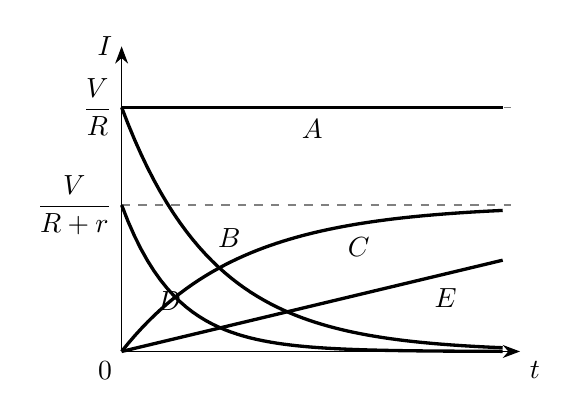
\begin{tikzpicture}[x=1.1cm, y=3.1cm]
  \draw[eje] (0,0) -- (4.6,0) node[below right]{$t$};
  \draw[eje] (0,0) -- (0,1.25) node[left]{$I$};
  \node[below left] at (0,0) {$0$};
  \draw[dashed, gray] (0,1) -- (4.5,1);
  \draw[dashed, gray] (0,0.6) -- (4.5,0.6);
  \node[left] at (0,1) {$\dfrac{V}{R}$};
  \node[left] at (0,0.6) {$\dfrac{V}{R+r}$};
  \draw[very thick] (0,1) -- (4.4,1);
  \node[below] at (2.2,0.99) {$A$};
  \draw[very thick] plot[domain=0:4.4, samples=60] (\x, {exp(-0.95*\x)});
  \node[above right] at (1.0,{exp(-0.95*1.0)}) {$B$};
  \draw[very thick] plot[domain=0:4.4, samples=60] (\x, {0.6*(1-exp(-0.75*\x))});
  \node[below right] at (2.5,{0.6*(1-exp(-0.75*2.5))}) {$C$};
  \draw[very thick] plot[domain=0:4.4, samples=60] (\x, {0.6*exp(-1.6*\x)});
  \node[left] at (0.8,{0.6*exp(-1.6*0.8)+0.04}) {$D$};
  \draw[very thick] plot[domain=0:4.4, samples=60] (\x, {0.085*\x});
  \node[below right] at (3.5,{0.085*3.5}) {$E$};
\end{tikzpicture}
\end{document}
